%!TEX root = ../../main.tex

\chapter{Das Monty-Hall-Standard-Problem} \label{chap:monty-hall-standard}

Aufgrund von nicht eindeutig ausformulierten Regeln befanden einige Wissenschaftler die Aufgabe für nicht eindeutig lösbar und es wurde eine Neuformuliering des
Ziegenproblems vorgeschlagen. Diese abgeänderte Version der Aufgabe wurde als das Monty-Hall-Standard-Problem bekannt. Weiterhin sollte das Problem zur gleichen
Lösung führen, wie die, die von Marilyn vos Savant vorgelegt wurde. Zusätzlich sollen aber nun weitere Zusatzinformationen gegeben werden, welche erfahrungsbezogene Antworten ungültig
machen, und darüber hinaus soll die aktuelle Spielsituation berücksichtigt werden. (\cite{Mueser:1999})

\section{Definition der Spielregeln}

Aufgeteilt in Einzelschritte ergeben sich dann die folgenden Regeln für den Spieler und den Moderator. (\cite{Savant:2001})
\begin{enumerate}
    \item Ein Auto und zwei Ziegen werden zufällig auf drei Tore verteilt.
    \item Zu Beginn des Spiels sind alle Tore verschlossen, sodass Auto und Ziegen nicht sichtbar sind.
    \item Der Kandidat, dem die Position des Autos völlig unbekannt ist, wählt ein Tor aus, das aber vorerst verschlossen bleibt.
    \item Der Moderator öffnet ein weiteres ,,Ziegentor''\begin{itemize}
              \item Fall A: Hat der Kandidat das Tor mit dem Auto gewählt, öffnet der Moderator eines der beiden anderen Tore, hinter dem sich immer eine Ziege befindet.
                    Der Moderator hat dabei die freie Wahl. Wie er diese Wahl trifft wird in den folgenden Varianten durch Zusatzannahmen festgelegt.
              \item Fall B: Hat der Kandidat ein Tor mit einer Ziege gewählt, \textit{muss} der Moderator das Tor nehmen, hinter dem die andere Ziege steht.
          \end{itemize}
    \item Der Moderator bietet dem Kandidaten an, seine Entscheidung zu überdenken und das andere ungeöffnete Tor zu wählen.
    \item Das letztendlich vom Kandidaten gewählte Tor wird geöffnet und er erhält das Objekt, dass sich hinter dem Tor befindet.
\end{enumerate}

\section{Das Verhalten des Moderators}

Die folgenden Varianten unterscheiden sich nur darin, welches Tor der Moderator öffnet, wenn der Kandiadat direkt das richtige Tor auswählt (Regel 4, Fall A). Beispielsweise kann der Moderator rein zufällig entscheiden oder er macht es sich einfach und öffnet das Tor, das am nächsten zu ihm steht. Wir werden sehen, dass sich für verschiedene Annahmen über das Verhalten des Moderators die Gewinnwahrscheinlichkeit beim Wechseln ändert.

% ------ ausgeglichener Moderator

\subsection{Der Moderator handelt ausgeglichen}

Für die folgende Erklärung werden die Fälle betrachtet, bei denen der Spieler zu Beginn immer Tor 1 wählt. Alle anderen Fälle können analog erklärt werden.

Es wird die Zusatzannahme getroffen, das der Moderator rein zufällig entscheidet, welches Tor er gerne öffnen möchte. Wählt der Kandidat jedoch zuerst ein Tor mit einer Ziege, so hat der Moderator keine andere Wahl, als das andere Ziegentor zu öffnen. (\cite{Krauss:2003})

\subsubsection{Tabellarische Lösung}

\begin{tabular}[h]{|c|c|c|c|c|c|}
    \hline
    \textbf{Fall} & \textbf{Tor 1} & \textbf{Tor2} & \textbf{Tor3} & \textbf{Wahl des Moderator} & \textbf{Gewinn beim} \\
    \hline
    \multicolumn{6}{|c|}{\textit{der Moderator möchte Tor 2 öffnen} }                                                   \\
    \hline
    1             & Auto           & Ziege         & Ziege         & Tor 2                       & Bleiben              \\
    2             & Ziege          & Auto          & Ziege         & Tor 3, da Tor 2 Auto        & Wechseln             \\
    3             & Ziege          & Ziege         & Auto          & Tor 2                       & Wechseln             \\
    \hline
    \multicolumn{6}{|c|}{\textit{der Moderator möchte Tor 3 öffnen}
    }                                                                                                                   \\
    \hline
    4             & Auto           & Ziege         & Ziege         & Tor 3                       & Bleiben              \\
    5             & Ziege          & Auto          & Zeige         & Tor 3                       & Wechseln             \\
    6             & Ziege          & Ziege         & Auto          & Tor 2, da Tor 3 Auto        & Wechseln             \\
    \hline
\end{tabular}

Zur Auswertung werden die Fälle mit einander verglichen, bei denen Wechseln bzw. Bleiben zum Gewinn führt.
Dabei sieht man, dass der Kandidat in 4 der 6 Fälle das Auto durch den Wechsel findet (Fälle 2, 3, 5 und 6). In den anderen Fällen (1 und 4) würde der Kandidat das Auto gewinnen, wenn er auf seiner ersten Wahl beharrt.

Somit liegt die Wahrscheinlichkeit, dass der Kandidat das Auto durch Wechseln findet bei $P_W(Auto) = \frac{2}{3}$.

\subsubsection{Mathematische Lösung}

Bei dieser und allen anderen Varianten sind die A-priori-Wahrscheinlichkeiten $P(G_i)$, dass sich hinter dem Tor $i$ das Auto befindet, gleich. Deshalb lassen sich diese beim Satz von Bayes (\autoref{equ:bayes}) kürzen, damit später die vereinfachte Version (\autoref{equ:bayes_simpl}) verwendet werden kann:

\begin{equation*}
    P(G_1)=P(G_2)=P(G_3)=\frac{1}{3}
\end{equation*}

Wie zuvor beschrieben wählt der Kandidat Tor 1 aus und wechselt, nach dem Öffnen eines Tores durch den Moderator, zu dem nicht zuvor ausgewähltem Tor.

Folgende bedingte Wahrscheinlichkeiten können bei dieser Annahme definiert werden, falls der Moderator das 3. Tor öffnet (das Gleiche gilt analog für Tor 2):
\begin{align*}
    P(M_3 | G_1) & = \frac{1}{2} \\
    P(M_3 | G_2) & = 1           \\
    P(M_3 | G_3) & = 0
\end{align*}

\textbf{Kurze Erläuterung dieser Beziehungen:} $P(M_3 | G_1)$ beschreibt die Wahrscheinlichkeit dass falls der Gewinn hinter Tor 1 steht, der Moderator Tor 3 öffnet. Da in diesem Fall der Moderator rein zufällig aus zwei Optionen wählt, liegt diese Wahrscheinlichkeit bei $\frac{1}{2}$. Steht das Auto hinter dem Zweiten Tor, hat der Moderator keine andere Wahl, als Tor 3 zu öffnen. Deshalb liegt $P(M_3 | G_2)$ bei $1$. Wenn das Auto hinter Tor 3 steht, kann Tor 3 nicht geöffnet werden. $P(M_3 | G_3)$ muss $0$ sein.

Unter der Anwendung des Satzes von Bayes (\autoref{equ:bayes_simpl}) können die bedingten Wahrscheinlichkeiten, dass hinter den jeweiligen Toren das Auto steht unter der Vorraussetzung, dass Tor 3 vom Moderator geöffnet wurde, bestimmt werden:

\begin{align*}
    P(G_i | M_3) & = \frac{P(M_3 | G_i)}{P(M_3 | G_1) +
    P(M_3 | G_2) + P(M_3 | G_3)}                                       \\
    P(G_1 | M_3) & = \frac{\frac{1}{2}}{\frac{1}{2}+1+0} = \frac{1}{3} \\
    P(G_2 | M_3) & = \frac{1}{\frac{3}{2}} = \frac{2}{3}               \\
    P(G_3 | M_3) & = 0
\end{align*}

Somit ist bewiesen, dass die Gewinnwahrscheinlichkeit von anfangs $\frac{1}{3}$ durch Wechseln auf $P_W(Auto) = \frac{2}{3}$ erhöht.

Dieses Szenario entspricht auch dem klassischen Monty-Hall-Problem, wie es von vos Savant vorgestellt wurde.

% ------ fauler Moderator

\subsection{Der Moderator handelt faul}

Für die folgende Erklärung werden die Fälle betrachtet, bei denen der Spieler zu Beginn immer Tor 1 wählt. Alle anderen Fälle können wieder analog erklärt werden.

Nun wird jedoch angenommen, der Moderator sei faul und öffne immer das Tor, das am nächsten zu ihm steht (Beispielsweise das Tor 3). Befindet sich hinter dem ersten Tor eine Ziege hat er jedoch wieder keine andere Wahl, als das zweite Ziegentor zu öffnen. (\cite{Rosenthal:2008})

\subsubsection{Tabellarische Lösung} \label{subsubsec:table_faul}

\begin{tabular}[h]{|c|c|c|c|c|c|}
    \hline
    \textbf{Fall} & \textbf{Tor 1} & \textbf{Tor2} & \textbf{Tor3} & \textbf{Wahl des Moderator} & \textbf{Gewinn beim} \\
    \hline
    1             & Auto           & Ziege         & Ziege         & Tor 3                       & Bleiben              \\
    2             & Ziege          & Auto          & Ziege         & Tor 3                       & Wechseln             \\
    3             & Ziege          & Ziege         & Auto          & Tor 2, da Tor 3 Auto        & Wechseln             \\
    \hline
\end{tabular}

Die Tabelle Zeigt, dass die Wahrscheinlichkeit beim Wechseln zu gewinnen davon abhängt, welches Tor geöffnet wurde.

In den Fällen 1 und 2 öffnet der Moderator das Tor mit der Nummer 3. Nur in einem dieser zwei Fälle gewinnt der Spieler, wenn er wechselt. Das bedeutet die Siegeswahrscheinlichkeit durch Wechseln $P_W(Auto) = \frac{1}{2}$ beträgt, wenn Tor 3 geöffnet wurde.

Für den Fall, dass Tor 2 geöffnet wurde (Fall 3) sollte unter der Annahme des faulen Moderators klar sein, dass hinter Tor 3 der Gewinn steht (sonst hätte er ja dieses Tor geöffnet). Da dies nur den Fall 3 betrifft, bei dem durch Wechseln gewonnen wird, ist die Gewinnwahrscheinlichkeit, wenn der Kandidat wechselt hier $P_W(Auto) = 1$.

\subsubsection{Mathematische Lösung}

Durch die im Vorhinein festgelegten Bedingungen ergeben sich die folgende mögliche Situationen:
\begin{enumerate}
    \item Der Kandidat wählt das erste Tor. Der faule Moderator öffnet das für ihn nächste Tor, nämlich Tor 3.
    \item Der Kandidat wählt das erste Tor. Da hinter Tor 3 das Auto steht, muss der Moderator Tor 2 öffnen.
\end{enumerate}

Für die Erste Situation gelten folgende mathematischen Beziehungen:

\begin{align*}
    P(M_3 | G_1) = 1 \\
    P(M_3 | G_2) = 1 \\
    P(M_3 | G_3) = 0
\end{align*}

Durch Anwendung des Satz von Bayes (\autoref{equ:bayes_simpl}) ergeben sich folgende Wahrscheinlichkeiten:

\begin{align*}
    P(G_i | M_3) & = \frac{P(M_3 | G_i)}{P(M_3 | G_1) + P(M_3 | G_2) + P(M_3 | G_3)} \\
    P(G_1 | M_3) & = \frac{1}{1+1+0} = \frac{1}{2}                                   \\
    P(G_2 | M_3) & = \frac{1}{2}                                                     \\
    P(G_3 | M_3) & = 0                                                               \\
\end{align*}

Die Gewinnwahrscheinlichkeit beim Wechseln entspricht somit $P_W(Auto) = P(G_2 | M_3) = \frac{1}{2}$

Für die zweite Situation, dass Tor 2 geöffnet wird, sehen die Beziehungen anders aus:

\begin{align*}
    P(M_2 | G_1) = 0 \\
    P(M_2 | G_2) = 0 \\
    P(M_2 | G_3) = 1
\end{align*}

Mit dem Satz von Bayes (\autoref{equ:bayes_simpl}) lassen sich nun die bedingte Wahrscheinlichkeit dafür bestimmen, dass das Auto hinter einem Tor steht, unter der Vorraussetzung, dass Tor 2 geöffnet wurde:

\begin{align*}
    P(G_i | M_3) & = \frac{P(M_3 | G_i)}{P(M_3 | G_1) + P(M_3 | G_2) + P(M_3 | G_3)} \\
    P(G_1 | M_2) & = \frac{0}{0+0+1} = 0                                             \\
    P(G_2 | M_2) & = 0                                                               \\
    P(G_3 | M_2) & = 1                                                               \\
\end{align*}

Die Gewinnwahrscheinlichkeit beim Wechseln entspricht hier $P_W(Auto) = P(G_3 | M_2) = 1$

\subsubsection{Mittelwertberechnung}

Der Mittelwert der Gewinnwahrscheinlichkeiten beim Wechseln lässt sich durch den gewichteten Mittelwert bestimmen. Dabei werden die verschiedenen Werte mit den jeweiligen relativen Häufigkeiten multipliziert und summiert.

Laut der Tabelle in \ref{subsubsec:table_faul} Tabellarische Lösung beträgt in zwei von drei Fällen $P_W(Auto) = \frac{1}{2}$ und in einem Fall $1$. Der gewichtete Mittelwert entspricht dadurch:

\begin{equation}
    \label{equ:mittelwert_faul}
    \overline{P_W(Auto)} = \frac{2}{3} \cdot \frac{1}{2} + \frac{1}{3} \cdot 1 = \frac{2}{3}
\end{equation}

Somit entspricht auch die Lösung unter dieser Annahme zumindest im Mittel der ursprünglichen Erklärung von vos Savant.

% ------ unausgeglichener Moderator

\subsection{Der Moderator handelt unausgeglichen}

Hierfür muss folgende Zusatzannahme getroffen werden. Hat der Kandidat zuerst das Tor mit dem Auto ausgewählt, entscheidet sich der Moderator mit einer Wahrscheinlichkeit von $p$
für das Tor mit der höchstmöglichen Nummer. Dadurch lässt sich folgern, dass die Wahrscheinlichkeit, dass der Moderator das Tor mit der kleinstenmöglichen Nummer öffnet $1 - p$ beträgt.

\subsubsection{Mathematische Lösung}

Die bedingten Wahrscheinlichkeiten, dass der Moderator das letzte Tor öffnet, unter der Bedingung, dass der Gewinn hinter den jeweiligen Toren steckt lauten:

\begin{align*}
    P(M_3 | G_1) & = p \\
    P(M_3 | G_2) & = 1 \\
    P(M_3 | G_3) & = 0
\end{align*}

Mit dem Satz von Bayes (\autoref{equ:bayes_simpl}):

\begin{align*}
    P(G_i | M_3) & = \frac{P(M_3 | G_i)}{P(M_3 | G_1) + P(M_3 | G_2) + P(M_3 | G_3)} \\
    P(G_1 | M_3) & = \frac{p}{p+1+0} = \frac{p}{p+1}                                 \\
    P(G_2 | M_3) & = \frac{1}{p+1}                                                   \\
    P(G_3 | M_3) & = 0                                                               \\
\end{align*}

Dieselben Betrachtungen können auch für das Tor mit der kleinstenmöglichen Nummer getroffen werden:

\begin{align*}
    P(M_2 | G_1) & = 1 - p \\
    P(M_2 | G_2) & = 0     \\
    P(M_2 | G_3) & = 1
\end{align*}

\begin{align*}
    P(G_i | M_2) & = \frac{P(M_2 | G_i)}{P(M_2 | G_1) + P(M_2 | G_2) + P(M_2 | G_3)} \\
    P(G_1 | M_2) & = \frac{1-p}{(1-p)+0+1} = \frac{1-p}{2-p}                         \\
    P(G_2 | M_2) & = 0                                                               \\
    P(G_3 | M_2) & = \frac{1}{2-p}                                                   \\
\end{align*}

Der unausgeglichene Moderator lässt sich als Verallgemeinerung der vorhergegangen Zusatzannahmen über das Verhalten des Moderators betrachten. So kann man die Gewinnwahrscheinlichkeiten einfach durch Einsetzten des richtigen $p$ ableiten.
Bei dem ausgeglichenen Moderator wäre $p = \frac{1}{2}$ und bei dem faulen Moderator $p = 1$.  (\cite{Rosenthal:2008})

\subsubsection{Mittelwertberechnung}

Da für $p = \frac{1}{2}$ die Gewinnwahrscheinlichkeit beim Wechseln $\frac{2}{3}$ betrag und bei $p = 1$ dies für den Mittelwert auch galt, wollen wir versuchen, ob wir auch allgemein diesen Mitelwert für alle $p$ ermitteln können. Dieser entspricht dem gewichteten Mittelwert

\label{equ:mittelwert}
\begin{equation}
    \begin{split}
        \overline{P_W(Auto)} & = P(G_2 | M_3) \cdot x + P(G_3 | M_2) \cdot y    \\
        & = \frac{1}{p+1} \cdot x + \frac{1}{2-p} \cdot y,
    \end{split}
\end{equation}

wobei es sich bei $x$ bzw. $y$ um die relative Häufigkeit, dass der Moderator Tor 3 bzw. Tor 2 öffnet, handelt. Um diese zu bestimmen, betrachten wir noch einmal die speziellen Fälle ausgeglichen und faul (vgl. \autoref{equ:mittelwert_faul}):

\begin{align*}
    p = \frac{1}{2} & \Rightarrow \overline{P_W(Auto)} = \frac{2}{3} \cdot \frac{1}{2} + \frac{2}{3} \cdot \frac{1}{2} = \frac{2}{3} \\
    p = 1           & \Rightarrow \overline{P_W(Auto)} = \frac{1}{2} \cdot \frac{2}{3} + 1\cdot \frac{1}{3} = \frac{2}{3}
\end{align*}

Die Werte für $x$ und $y$ lassen sich in Abhängigkeit von $p$ in einer Tabelle abtragen:

\begin{center}
    \begin{tabular}[h]{|c|c|c|}
        \hline
        \textbf{$p$}  & \textbf{$x$}  & \textbf{$y$}  \\
        \hline
        $\frac{1}{2}$ & $\frac{1}{2}$ & $\frac{1}{2}$ \\
        $1$           & $\frac{2}{3}$ & $\frac{1}{3}$ \\
        \hline
    \end{tabular}
\end{center}

Trägt man die Punkte in ein Koordinatensystem und legt Geraden hindurch (\autoref{fig:x-y}), lassen sich für x und y folgende Funktionen ablesen:

\begin{figure}[hbtp]
    \centering
    \captionsetup{name=Abb., justification=centering, format=nolinebreak}
    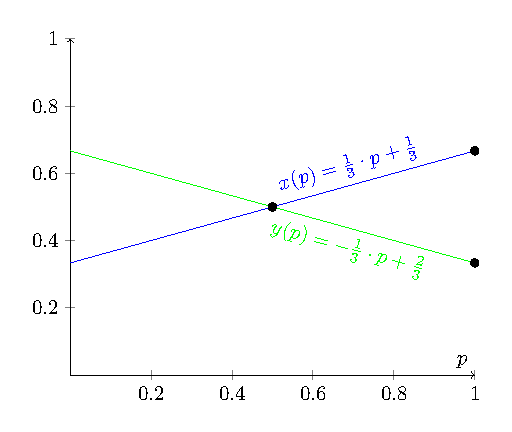
\includegraphics[width=0.3\textwidth]{tex/graph.pdf}
    \caption{Bestimmung $x(p)$ und $y(p)$} \label{fig:x-y}
\end{figure}

\begin{align*}
    x(p) & = \frac{1}{3} \cdot p + \frac{1}{3} = \frac{p + 1}{3} \\
    y(p) & = -\frac{1}{3} \cdot p + \frac{2}{3} = \frac{2-p}{3}
\end{align*}

Schlussendlich kann allgemein der Mittelwert nach der Formel \ref{equ:mittelwert} bestimmt werden:

\begin{align*}
    P_W & = P(G_2 | M_3) \cdot x(p) + P(G_3 | M_2) \cdot y(p)                                       \\
        & = \frac{1}{p+1} \cdot \frac{p + 1}{3} + \frac{1}{2-p} \cdot \frac{2 - p}{3} = \frac{2}{3}
\end{align*}

Somit haben wir gezeigt, dass unabhängig von $p$ (also egal ob der Moderator eine Türe in irgendeiner Weise bevorzugt) die Wahrscheinlichkeit das Auto durch Wechseln zu gewinnen zu mindest im Mittel $\frac{1}{3}$ beträgt.
